%%%%%%%%%%%%%%%%%%%%%%%%%%%%%%%%%%%%%%%%%
%
% (c) 2018 by Jennifer Laaser
%
% This work is licensed under the Creative Commons Attribution-NonCommercial-ShareAlike 4.0 International License. To view a copy of this license, visit http://creativecommons.org/licenses/by-nc-sa/4.0/ or send a letter to Creative Commons, PO Box 1866, Mountain View, CA 94042, USA.
%
% The current source for these materials is accessible on Github: https://github.com/jlaaser/quantum-exercises
%
%%%%%%%%%%%%%%%%%%%%%%%%%%%%%%%%%%%%%%%%%

\section*{Wavepackets\sectionmark{Wavepackets}}

\begin{questions}
\question Consider a Gaussian wavepacket travelling to the right. At $t=0$, its probability distribution might look like this:

	\vspace{0.1in}
	\centerline{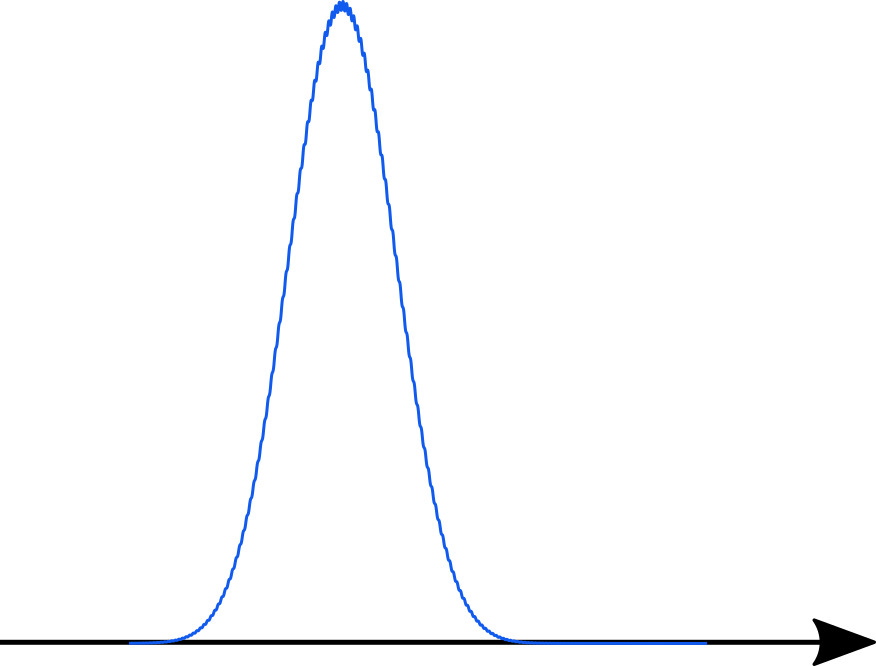
\includegraphics[width=0.6\textwidth]{includes/wavepackets-FIGURES/gaussian.jpg}}
	\vspace{0.1in} 
 
	\begin{parts}
		\part What feature of this plot (if any) gives you information about the uncertainty in the particle’s position? Mark it on the plot.

		\part What feature of this plot (if any) gives you information about the uncertainty in the particle’s momentum?  Mark it on the plot.
	\end{parts}

	\vspace{0.1in}
		\question On the plots below, predict what the wavepacket's probability distribution will look like at some time slightly after t=0 if the uncertainty in the momentum is...

	\vspace{0.2in}
	\begin{minipage}{0.5\textwidth}
		\centerline{... small?}\vspace{0.1in}
		
	\centerline{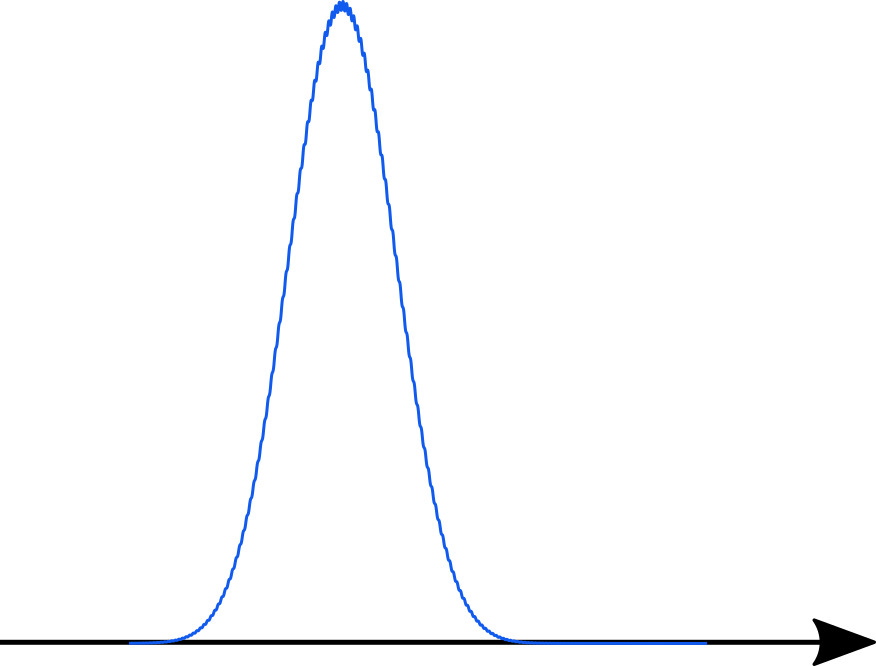
\includegraphics[width=0.8\textwidth]{includes/wavepackets-FIGURES/gaussian.jpg}}
	\end{minipage}
	\begin{minipage}{0.5\textwidth}
		\centerline{... large?}\vspace{0.1in}
		
	\centerline{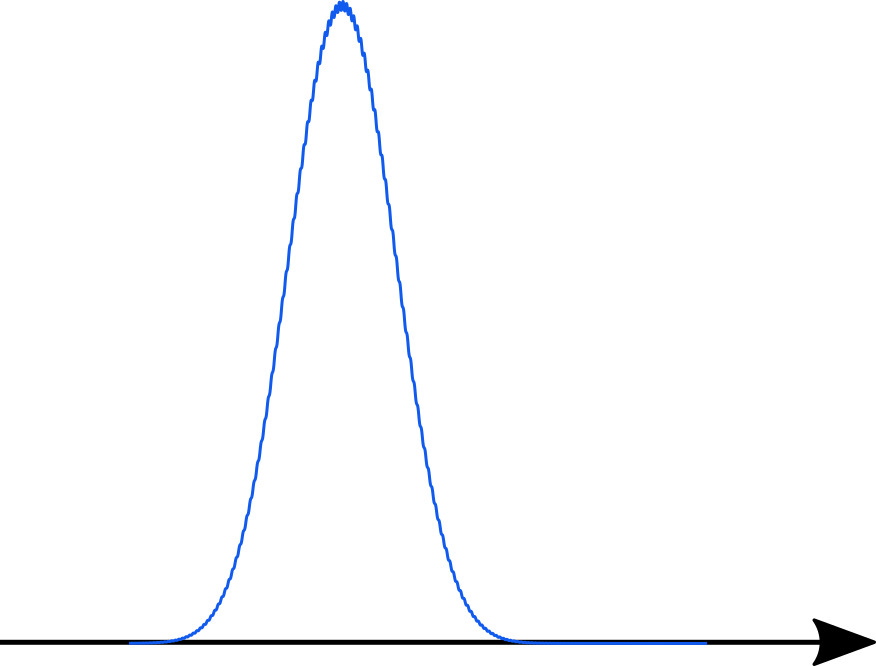
\includegraphics[width=0.8\textwidth]{includes/wavepackets-FIGURES/gaussian.jpg}}
	\end{minipage}
	
	\vspace{0.3in}
	
	\contdnewpg

\question The following plots show the propagation of two different wavepackets:

      	\vspace{0.2in}
	\begin{minipage}{0.5\textwidth}
	\centerline{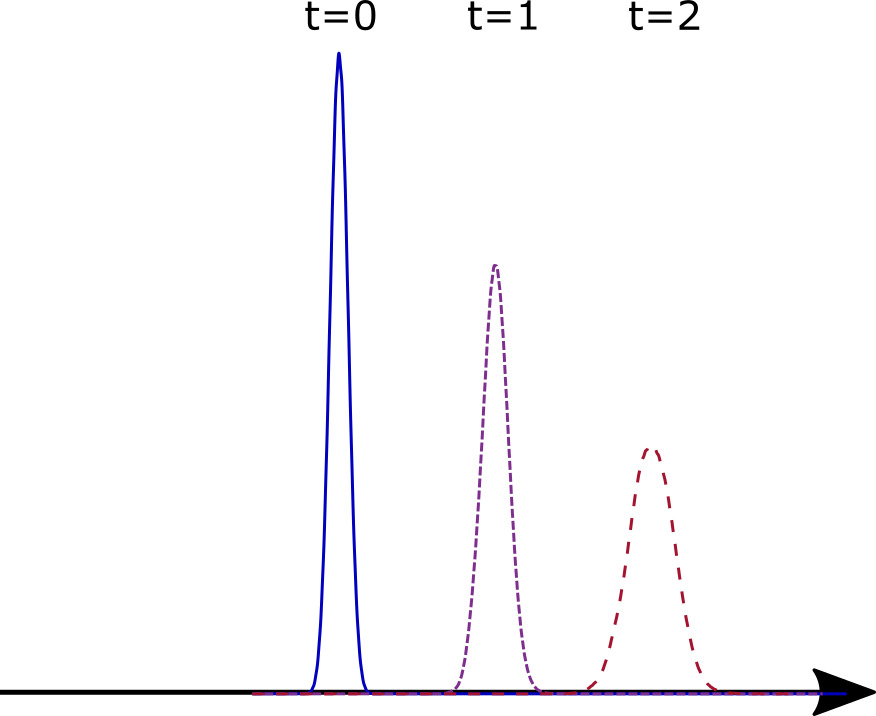
\includegraphics[width=0.8\textwidth]{includes/wavepackets-FIGURES/prop1.jpg}}
	\end{minipage}
	\begin{minipage}{0.5\textwidth}
	\centerline{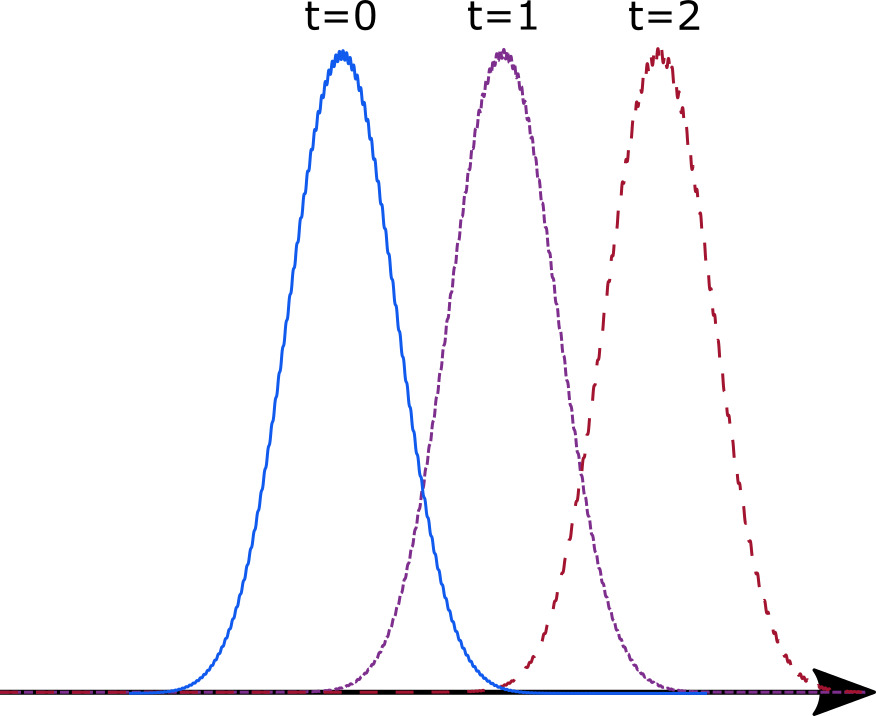
\includegraphics[width=0.8\textwidth]{includes/wavepackets-FIGURES/prop2.jpg}}
	\end{minipage}
	\vspace{0.1in}

Identify which wavepacket has the larger uncertainty in the position and which has the larger uncertainty in the momentum, and explain how your observations relate to the uncertainty principle:
	
	\vspace{3.25in}

\end{questions}
